\documentclass[conference]{IEEEtran}

\usepackage{cite}
\usepackage{amsmath,amssymb,amsthm}
\usepackage{booktabs}
\usepackage{algorithm}
\usepackage{algorithmic}
\usepackage{tikz}
\usetikzlibrary{positioning,fit}
\usepackage{pgfplots}
\pgfplotsset{compat=1.17}
\usepackage{graphicx}
\usepackage{url}

\begin{document}

\title{Do Learned Index Models Remember What You Deleted? Strong History Independence of the Serialized Model}

\author{\IEEEauthorblockN{Anubhav Pandey}
\IEEEauthorblockA{\textit{Department of Computer Science and Engineering}\\
\textit{Indian Institute of Technology Delhi}\\
New Delhi, India\\
cs5221136@iitd.ac.in\\
ORCID: 0009-0006-9755-5871}}

\maketitle

\begin{abstract}
Dynamic learned indexes delete a key by leaving a tombstone or a gap, and a later reader of that structure can recover the key.
On the full SOSD files, shipped dynamic PGM still stores a 16-byte tombstone after hundreds of later deletes, ALEX leaves the key in the payload after clearing an existence bit, and the LIPP sources we build against have no erase.
We take the serialized model Repr, the segment tables, error bound, modulus, and segmenter identity, to be strongly history independent when those bytes depend only on the keys that remain. The key arena and the anchor secret are outside that record. Packing the survivors and fitting a static PGM already meets that byte condition for one checkpoint. The splice is the live model a reader of Repr sees before that checkpoint.
A local splice that stops at the next old start key matches a fresh build on 4,000 fuzzer checks, on 100 deletes of each SOSD file, and after a 32-delete batch and a 20,000-operation mix. Mean delete time without the slide is 0.67 ms, 2.20 ms, 1.47 ms, and 7.61 ms on wiki, fb, books, and osm. The slowest of 512 deletes finishes 813, 125, 325, and 156 times sooner than a separate static PGM build. At modulus 4096, lookup on a fresh arena is 390 to 743 ns, or 1.68 to 2.00 times static PGM, and the model is 1.10 to 1.28 times static PGM except 2.37 times on wiki.
When the surviving keys are known, a rebuild names the deleted key for every exact structure we tried. Without that knowledge this index's window on the 200,000-key generators is 4.0 to 68.4 percent, localization among 999 decoys against a 0.1 percent draw. The 3.1 percent figure is static PGM on the squared keys.
\end{abstract}

\begin{IEEEkeywords}
learned indexes, history independence, indexing, data deletion, piecewise-linear approximation
\end{IEEEkeywords}

\section{Introduction}

A learned index replaces routing nodes with a model of the empirical CDF~\cite{kraska2018,ferragina2020pgm}.
Dynamic variants stay updatable by recording a tombstone, opening a gap, or leaving the fitted model in place, and a later reader of that structure can still recover the deleted key~\cite{ferragina2020pgm,ding2020alex,wu2021lipp}.
This paper is about the serialized model, not about whether a storage sanitizer already rewrote the key array~\cite{shastri2020,sarkar2023lethe,wagner2024dbsanitizer}.
A segment start key is often a raw key, and a tombstone is a stored record.
A segment that stores its intercept in the global rank space cannot be left alone after a delete.
Three segments with relative counts $(4,3,5)$ become $(3,3,5)$ when a key in the first segment is removed, and the stored suffix is untouched.
The same segments stored as global intercepts $(0,4,7)$ become $(0,3,6)$: both later fields move, and a local splice cannot match a rebuild.
A history-independent B-tree does not have that coupling~\cite{bender2016}.
A frequency tree that keeps two copies is fitting node depth to a frequency prediction, not segmenting a CDF.
The model here stores a count and a segment-local intercept so the suffix can stay.
Fig.~\ref{fig:attack} draws that contrast on one deleted key.

\begin{figure*}[t]
\centering
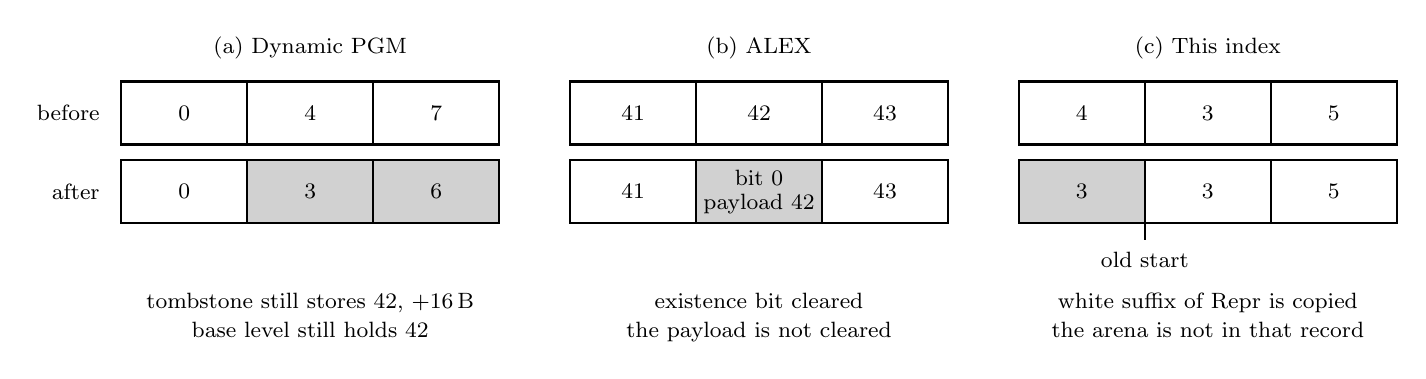
\begin{tikzpicture}[x=1mm, y=1mm, font=\footnotesize]
  \node[anchor=east] at (14.5,14) {before};
  \node[anchor=east] at (14.5,4) {after};
  \node[anchor=south] at (40,19.6) {(a) Dynamic PGM};
  \node[anchor=south] at (97,19.6) {(b) ALEX};
  \node[anchor=south] at (154,19.6) {(c) This index};

  \fill[black!18] (32,0) rectangle (64,8);
  \draw[thick] (16,0) rectangle (64,8);
  \foreach \x in {32,48} \draw[thick] (\x,0) -- (\x,8);
  \node at (24,4) {0};
  \node at (40,4) {3};
  \node at (56,4) {6};
  \draw[thick] (16,10) rectangle (64,18);
  \foreach \x in {32,48} \draw[thick] (\x,10) -- (\x,18);
  \node at (24,14) {0};
  \node at (40,14) {4};
  \node at (56,14) {7};

  \fill[black!18] (89,0) rectangle (105,8);
  \draw[thick] (73,0) rectangle (121,8);
  \foreach \x in {89,105} \draw[thick] (\x,0) -- (\x,8);
  \node at (81,4) {41};
  \node[align=center] at (97,4) {bit 0\\[-0.3mm]payload 42};
  \node at (113,4) {43};
  \draw[thick] (73,10) rectangle (121,18);
  \foreach \x in {89,105} \draw[thick] (\x,10) -- (\x,18);
  \node at (81,14) {41};
  \node at (97,14) {42};
  \node at (113,14) {43};

  \fill[black!18] (130,0) rectangle (146,8);
  \draw[thick] (130,0) rectangle (178,8);
  \foreach \x in {146,162} \draw[thick] (\x,0) -- (\x,8);
  \node at (138,4) {3};
  \node at (154,4) {3};
  \node at (170,4) {5};
  \draw[thick] (146,0) -- (146,-2.2);
  \node[anchor=north] at (146,-2.4) {old start};
  \draw[thick] (130,10) rectangle (178,18);
  \foreach \x in {146,162} \draw[thick] (\x,10) -- (\x,18);
  \node at (138,14) {4};
  \node at (154,14) {3};
  \node at (170,14) {5};

  \node[anchor=north, align=center, text width=46mm] at (40,-7.6)
    {tombstone still stores 42, $+16$\,B\\[0.4mm]base level still holds 42};
  \node[anchor=north, align=center, text width=46mm] at (97,-7.6)
    {existence bit cleared\\[0.4mm]the payload is not cleared};
  \node[anchor=north, align=center, text width=46mm] at (154,-7.6)
    {white suffix of Repr is copied\\[0.4mm]the arena is not in that record};
\end{tikzpicture}

\caption{One deleted key, drawn as the three segments in the introduction.
(a) Global intercepts $(0,4,7)$ become $(0,3,6)$: the later fields move.
The tombstone still stores 42, and the base level still holds it.
(b) ALEX clears an existence bit and leaves 42 in the payload.
(c) Relative counts $(4,3,5)$ become $(3,3,5)$.
The splice stops at the next old start, the white suffix of the segment table is copied, and those Repr bytes match a rebuild.
The key arena is not in Repr.}
\label{fig:attack}
\end{figure*}

This paper asks four questions.
\begin{enumerate}
\item How much do shipped dynamic learned indexes reveal about a deleted key to a reader who holds one snapshot?
\item Can a local splice of that serialized model match a fresh build before the next packed-key static-PGM checkpoint? The key array is outside that record.
\item What lookup, space, and delete cost does that representation pay against static PGM, on the SOSD files rather than on a cache-resident pilot?
\item What leakage remains for a reader who holds the snapshot from before the delete and the snapshot from after it?
\end{enumerate}

Strong history independence asks for a representation that is the same for every update sequence that produces the same contents~\cite{naor2001,hartline2005,blelloch2007}.
Applied to the serialized model, deleting $k$ has to yield the bytes of a fresh build on the surviving keys.
The process arena is a separate layout: a checkpoint writes the model and then the live keys packed in rank order, and holes in the process arena are outside that checkpoint.
An attacker who already knows the surviving keys and sees one snapshot learns nothing further about $k$.
Any exact deterministic structure changes when $k$ is removed, so a reader who holds the snapshot from before and the snapshot from after, and who can test candidates, can often name $k$.
A concurrent preprint gives strong history independence for frequency-based learning-augmented trees by keeping a second copy of the structure~\cite{goyal2025}.
That work fits node depth to a frequency prediction, on a static workload, and it does not segment a CDF.

The contributions are:
\begin{enumerate}
\item A single-snapshot account of stock dynamic PGM and ALEX on generators and on the full SOSD files.
\item A relative-count piecewise-linear splice of $\mathrm{Repr}$ that stops at the next old start key and matches a rebuild before the next packed-key static-PGM checkpoint.
\item Lookup, space, and delete cost of that live model against static PGM on wiki, fb, books, and osm.
\item A two-snapshot measurement: known-survivor rebuild identification is $100\%$ for every exact structure we tried, and Table~\ref{tab:t2} is localization among decoys, not hiding.
\end{enumerate}

\section{Related work}

PGM, ALEX, LIPP, RadixSpline, and the RMI are the CDF indexes this paper starts from, and SOSD is the measurement standard those papers use~\cite{ferragina2020pgm,ding2020alex,wu2021lipp,kipf2020spline,kraska2018,kipf2019sosd}.
PGM stores an intercept in the global rank space and, in the dynamic structure, deletes by inserting a tombstone under the logarithmic method.
ALEX places keys in gapped arrays and erases by shifting a key into a slot and clearing an existence bit.
LIPP's paper removes a key by marking the entry \texttt{NULL} and retaining the gap~\cite{wu2021lipp}.
None of these layouts requires the serialized model after a local edit to equal a fresh static build.

Naor and Teague, Hartline et al., and Blelloch and Golovin defined history independence~\cite{naor2001,hartline2005,blelloch2007}.
A deterministic build already satisfies the definition once the previous bytes are thrown away, so the systems question is whether a local edit can produce those bytes without a full refit.
Bender et al.\ give a history-independent packed-memory array and a cache-oblivious B-tree, and they separate one observation from many~\cite{bender2016}.
Their packed-memory layout is the logarithmic baseline for moving keys.
We cut the key array at the model's anchors and do not use their density thresholds.
The hash-promotion tree is only a second exact object for the byte checks.

Goyal, Sridhar, and Zheng give strong history independence for skip lists, treaps, and B-treaps whose depth follows a frequency prediction, by thresholding and by pairing two copies~\cite{goyal2025}.
Pairing costs about twice the space and up to twice the search.
This index is a relative-count streaming PLA with those cuts, so a local splice equals \texttt{Build} on the survivors, without a second copy and at the space in Table~\ref{tab:anchor}.
Later updatable learned indexes are out of scope: this paper measures shipped delete artifacts, not update throughput.

Schuster et al.\ show that a live learned index leaks co-tenant key distributions through timing~\cite{schuster2025}.
Kurmanji et al.\ study unlearning for cardinality estimation and related neural components, and they exclude indexes~\cite{kurmanji2024}.
DynaMind adjusts a learned index after deletes so that prediction error stays small~\cite{dynamind2026}.
Accuracy after unlearning is a different goal from byte-equivalence to a rebuild.
Differentially private and TEE-backed learned indexes hide query patterns or plaintext~\cite{du2024dp,cao2025letindex,wang2025sls}.
Yang, Kornaropoulos, and Cheng attack the availability of ALEX and PGM~\cite{yang2024}.
An exposed anchor secret is the same kind of availability issue: it lets an adversary force long refits, and it does not change the canonical bytes of the resulting set.

Content-defined chunking cuts a stream where a hash of the content hits a mask, so an edit rewrites bytes only until the next cut~\cite{muthitacharoen2001lbfs}.
The anchors in Section~\ref{sec:design} are that rule applied to keys, with a secret mixed in.

\section{Threat model}
\label{sec:threat}

A learned index scheme is $(\mathrm{Build},\mathrm{Upd},\mathrm{Repr})$.
$\mathrm{Repr}$ is the segment tables, the error bound, the anchor modulus, and the segmenter identity.
It leaves out the anchor secret and the key array.
If a disk image still contains the key array, erasure has already failed in storage~\cite{sarkar2023lethe,wagner2024dbsanitizer}, and the question here is what the model retains once that array has been rewritten.
A checkpoint writes $\mathrm{Repr}$ and then the live keys packed in rank order.
The delete slides the later keys of the piece one slot left and does not clear the vacated tail.
When the deleted key was not last in its piece, that tail holds a surviving key, the one just copied left.
When the deleted key was last in its piece, the tail still holds it.
The timed tables clear that tail with one store. A core dump of that path does not keep the deleted key in the vacated slot.
Neither byte is written into the checkpoint.
ALEX's retained payload is inside the structure erase returns.
Strong history independence here is a live-model byte invariant on $\mathrm{Repr}$.
A checkpoint that discards the live model and fits a static PGM on the packed keys already meets that invariant for the durable record.
The splice is the live model before that checkpoint.
A reader of one snapshot may hold only $\mathrm{Repr}$, or $\mathrm{Repr}$ followed by the live keys packed in rank order. Holes in the process arena are outside both.
Logs, the buffer pool, and freed pages are outside both, including after a storage-layer wipe~\cite{sarkar2023lethe,wagner2024dbsanitizer}.

Let $S(\mathrm{Ops})$ be the key set produced by an update sequence.
For a fixed secret, the scheme is strongly history independent when equal key sets produce equal bytes:
\[
\begin{aligned}
&S(\mathrm{Ops}_1)=S(\mathrm{Ops}_2) \\
&\quad\implies
\mathrm{Repr}(\mathrm{Upd}^*(\mathrm{Ops}_1))
=
\mathrm{Repr}(\mathrm{Upd}^*(\mathrm{Ops}_2)).
\end{aligned}
\]
Exact unlearning is the one-step case: the bytes after deleting $k$ equal $\mathrm{Repr}(\mathrm{Build}(S\setminus\{k\}))$.
Under that equality, a one-snapshot attacker who already knows the surviving keys learns nothing further about $k$.

T1 is one snapshot.
T2 is the pair of snapshots around one deletion.
T3, lookup timing for a co-tenant, is the attack in Schuster et al.~\cite{schuster2025} and is not measured here.
We separate two T1 statistics.
Recovery means the deleted key is still stored as a tombstone or a payload.
Window top-1 is the expected accuracy of a uniform draw among 1{,}000 candidates that fall in the key interval the snapshot names, against a $0.1\%$ chance.
A window statistic is localization, the accuracy of guessing among the candidates that land in the named interval, which is a different statistic from reading the key out of a slot.

Every generator attack uses 200{,}000 keys, 1{,}000 deletes, and 1{,}000 candidates, one of which is the deleted key.
The other 999 are keys drawn from the same array, skipping the deleted position, so every candidate is a key the workload could have stored.
Chance for a uniform draw among the 1{,}000 is $0.1\%$, and advantage over chance is the top-1 rate divided by that $0.1\%$.

For a stale PGM model the key is removed from the array and the fitted segments are left as they were.
The attacker names the segment whose key range contains the prediction, then draws the candidates that fall in that range.
If the largest jump in the stale predictions lands on the deleted rank, the top-1 contribution of that trial is $1$.
Otherwise it is one over the number of candidates inside the segment, which is the accuracy of guessing uniformly among them.
Segment-start exposure is the fraction of deletes whose deleted key equals a stored segment start of the stale model.
On books, fb, osm, and wiki that fraction was $0$, $1.7\%$, $0.2\%$, and $0.2\%$ (Table~\ref{tab:t1}, Start).
It is not the leaf count of this index.
The fb generator has $2{,}596$ leaves in this index, which is a different segment table.
Exact-rank hits, the jump landing on the deleted position, were $0.8\%$ (books), $2.7\%$ (fb), $0.9\%$ (osm), $1.4\%$ (wiki), and $100\%$ on $i^{2}$.
The window rates in Table~\ref{tab:t1} are larger because the segment is a wide interval: knowing the segment is already far above naming one key out of 1{,}000.

For ALEX the same candidate draw is restricted to the node the shift rule names.
Payload retention is scored separately, by reading the payload slot after the existence bit is cleared.
On the generators the node maximum stayed equal to the deleted key on $13.2\%$ of books probes, $10.0\%$ of fb, $0.8\%$ of wiki, and none of osm.
That rate is not the ALEX column of Table~\ref{tab:t1}.

The two-snapshot attacker holds the segment tables from before the delete and from after it.
A candidate scores when it is the unique key whose removal takes one table to the other, or, when several candidates are consistent with the changed interval, as one over that number.
The exact-rebuild column is the attacker who already knows every surviving key and tests which missing key rebuilds the observed bytes.

\section{What one snapshot retains}
\label{sec:t1}

\subsection{Dynamic PGM}

In the PGM-index code, erase inserts an item whose value is the tombstone, and the item remains until a later merge~\cite{ferragina2020pgm}.
On eight generated sets of 200{,}000 keys, a scan of the levels found the tombstone after all 1{,}000 deletes, and a copy of the key remained in the base level as well.
Each erase increased \texttt{size\_in\_bytes} by 16, the width of one stored item.
The same 16-byte growth, with the tombstone present, appears on the real SOSD files in Section~\ref{sec:eval}: all 8 deletes on wiki, fb, and books, and all 4 on osm, the deletes whose mean is Table~\ref{tab:sosd}.

A stale static model rarely names the deleted rank, except on the squared keys, and it does name the old segment.
The Window column of Table~\ref{tab:t1} is that top-1, against the $0.1\%$ chance above.
The hypothesis that a single snapshot localizes deleted keys at least $10\times$ above chance holds for this stale-model window on every generator we tried.
The tombstone itself is stronger than localization, because the key is still stored.
A window rate is localization, not a recovery; the tombstone and the ALEX payload are the recoveries.

\subsection{ALEX}

ALEX erase copies the next key into the slot and clears the existence bit.
It leaves the payload slot untouched, and it does not always update the node maximum when the erased key was that maximum~\cite{ding2020alex}.
With the key stored as its own payload, the payload remained in a cleared slot for $87$--$98\%$ of 250 probes on the four main generators (Table~\ref{tab:t1}).
Replaying the bulk-load rule $\max(\mathrm{predict}(k),\mathrm{last}+1)$ localizes the vacated slot to a short bracket.
On books, fb, osm, and wiki that window is $98.0\%$, $98.8\%$, $75.4\%$, and $72.3\%$, and on the squared keys it is $30.5\%$ (Table~\ref{tab:t1}, Shift).
The payload result is the one that recovers the key.

The same payload check on the full SOSD files retained the key on 20 of 20 erases for wiki (90{,}437{,}011 distinct keys), fb (200{,}000{,}000), books (199{,}999{,}999), and osm (800{,}000{,}000), after bulk loads of 17.3\,s, 74.4\,s, 44.0\,s, and 273\,s.
Node-maximum metadata was exposed on 0 of those 80 probes.
Zeroing every payload slot equal to the deleted key then left that key in neither the key slots nor the payload slots, on all 80 probes.
That write removes the raw key and leaves the gapped shifts and the fitted model.
On the generators, the same Shift column is the structural leak a payload write leaves behind.
The library's own erase does not zero the slot.
One million point queries drawn from those files, timed against static PGM in the same process, took 79\,ns, 604\,ns, 149\,ns, and 891\,ns, against paired PGM times of 224\,ns, 293\,ns, 260\,ns, and 441\,ns, so ALEX was $0.35\times$, $2.06\times$, $0.57\times$, and $2.02\times$ PGM.
None of those queries missed.
ALEX is faster than PGM on wiki and books, and about twice PGM on fb and osm.
The payload is still there after erase.
On the full files, dynamic PGM still held its first 20 tombstones after 800 further erases, and each of the 820 erases added 16 bytes.
The structure then occupied 1.45\,GB, 3.24\,GB, 3.21\,GB, and 12.9\,GB.

\subsection{LIPP}

The LIPP paper deletes by marking an entry \texttt{NULL} and keeping the gap~\cite{wu2021lipp}.
The sources this paper builds against expose insert, bulk load, and lookup, so we do not add a delete in this tree and then attack it as if it were LIPP.
A published index that cannot erase still holds every key it was built on.
Building a new index and discarding the old one does erase the key, and until that swap the published model is a function of the deleted key.

\begin{table}[t]
\caption{Single-snapshot leakage on 200{,}000-key generators.
PGM uses 1{,}000 deletes.
ALEX uses 250.
Tombstone is a key still stored in the data levels.
Rank is the stale model landing on the deleted position.
Window is the stale-PGM expected top-1 among 1{,}000 candidates, chance $0.1\%$.
Start is stale-PGM segment-start exposure.
ALEX is a payload still stored.
Shift is the ALEX bulk-load window.
This table is stock indexes. Byte identity of this paper's segment table is a separate check.}
\label{tab:t1}
\centering
\scriptsize
\begin{tabular}{@{}lrrrrrr@{}}
\toprule
Set & Tomb. & Rank & Window & Start & ALEX & Shift \\
\midrule
wiki   & 100\% & 1.4\% & 25.6\% & 0.2\% & 98.0\% & 72.3\% \\
fb     & 100\% & 2.7\% & 81.6\% & 1.7\% & 88.0\% & 98.8\% \\
books  & 100\% & 0.8\% & 14.3\% & 0 & 87.2\% & 98.0\% \\
osm    & 100\% & 0.9\% & 49.4\% & 0.2\% & 96.4\% & 75.4\% \\
\addlinespace
$i^{2}$ & 100\% & 100\% & 100\%  & 0 & 100\%  & 30.5\% \\
\bottomrule
\end{tabular}
\end{table}

\section{What two snapshots retain}
\label{sec:t2}

Exact history independence answers a reader who holds one snapshot: equal survivor sets produce equal model bytes, so that snapshot is the model a fresh build would publish.
It does not hide the deleted key from a reader who also holds the previous snapshot, or who knows the survivors and can rebuild.
The survivor set and the previous set differ by one key, so their canonical byte strings differ, and a reader who can rebuild both can test which candidate was removed.
Table~\ref{tab:t2} is that test on eight generators.
Static PGM and the anchored index land in the same band on every row.
The hash-promotion tree is higher, $81$--$86\%$, because a promotion boundary moves a larger fraction of the serialized nodes.
\begin{table}[t]
\caption{Two-snapshot window top-1 on 200{,}000-key generators.
One thousand candidates, survivor set unknown.
Exact rebuild is the attacker who knows the survivors and tests which candidate restores the observed bytes.
Chance is $0.1\%$.}
\label{tab:t2}
\centering
\footnotesize
\begin{tabular}{@{}lrrrr@{}}
\toprule
Set & PGM & SHI & HI tree & Exact \\
\midrule
books     & 6.3\% & 6.6\% & 84.5\% & 100\% \\
fb        & 69.5\% & 68.4\% & 81.4\% & 100\% \\
osm       & 29.0\% & 26.1\% & 84.8\% & 100\% \\
wiki      & 13.5\% & 11.8\% & 83.8\% & 100\% \\
\addlinespace
lognormal & 15.7\% & 14.7\% & 85.3\% & 100\% \\
uniform   & 9.3\% & 9.9\% & 86.0\% & 100\% \\
clustered & 16.8\% & 15.2\% & 85.7\% & 100\% \\
\addlinespace
$i^{2}$   & 3.1\% & 4.0\% & 81.5\% & 100\% \\
\bottomrule
\end{tabular}
\end{table}

When the attacker knows the survivor set and can rebuild, identification is $100\%$ for every exact scheme we tried, including this index, static PGM, and the hash-promotion tree (Table~\ref{tab:t2}).
Chance is $0.1\%$.
The $3.1\%$ cell is static PGM on the squared keys.
This index's smallest rate in the table is $4.0\%$.
With 999 decoys drawn from 200{,}000 keys, the rate mostly tracks how many of those decoys land in the named interval.

A two-snapshot mechanism that would hide the key needs a public grid or a quantile release that spends privacy budget, and this paper does not provide one.
Exact structures, history-independent or otherwise, leak the deleted key across two snapshots.

\section{A canonical piecewise-linear index}
\label{sec:design}

\subsection{Why the intercept has to be local}

A PGM segment stores an intercept in the global rank space and compresses those intercepts against $n$~\cite{ferragina2020pgm}.
Deleting one key changes every later rank, so every later stored intercept changes.
As in the introduction, a local count leaves the suffix in place and a global intercept does not.
A history-independent local delete therefore stores a count, or an intercept in the segment-local rank, rather than a position in the whole array.
The index here stores 16 bytes: the first key, a \texttt{float} slope with zero canonicalized to $+0$, a signed 16-bit intercept, and a 16-bit key count.
The count caps a segment at 65{,}535 keys.
The prediction inside a segment is $\mathrm{slope}\cdot(x-x_0)+\mathrm{intercept}$, and the intercept is that prediction at the first key, in the segment-local rank.
The global rank is the prefix sum of earlier counts plus that offset, so a later segment's stored fields do not depend on how many keys sit before it.
At $\varepsilon=16$ the hull keeps it within the error of local rank 0, so the 16-bit range does not end a segment on these files.
The fitter still refuses to store a clamped intercept, and it also ends a segment when the count would pass 65{,}535, when the $\varepsilon$-hull rejects the next key, or when the next key is an anchor.
The same rule is used by a full build and by a local delete.
The lookup window of width $\varepsilon$ is the window the fitter actually guaranteed.
Upper levels are another piecewise-linear model on the leaf start keys, with error $4$, and they use the same anchor modulus as the leaves.
Prefix sums and the lookup cache are not serialized.

When the gap and the product both fit in the 53-bit mantissa, the product is a double rounded to nearest.
Wider gaps use an integer product of the significand and the gap, rounded to nearest even, so a wide \texttt{uint64} range does not wrap a 64-bit position.
The exhaustive check below includes the double path and does not show that the two roundings are bit-identical.
The error window absorbed the difference on every audited key.
On a fresh index the keys sit in rank order in one arena, and the last step of lookup searches that arena at the predicted rank.
After a delete the same step searches inside the piece that holds the rank, and copies a window only when the error interval crosses a piece boundary.
Every key of the fresh arena was looked up: 90{,}437{,}011 wiki keys, 200{,}000{,}000 fb keys, 199{,}999{,}999 books keys, and 800{,}000{,}000 osm keys, 1{,}290{,}437{,}010 in all, and none missed.
After one delete of the middle key, every surviving key was looked up as well, 90{,}437{,}010, 199{,}999{,}999, 199{,}999{,}998, and 799{,}999{,}999 keys, and none missed.
The timed check after 1{,}024 deletes is one million probes on each file, all exact, and a separate pass over every survivor of a different 1{,}024-delete draw missed none.

\subsection{Anchors and local deletion}

An anchor is a key that must start a segment, $\mathrm{splitmix64}(x+s)\bmod M=0$, with $s$ absent from $\mathrm{Repr}$.
For a fixed secret the build is still a function of the key set, and the secret only limits cascade length.
An attacker who learns the secret can choose keys that avoid anchors and force long refits, which is an availability problem in the sense of Yang et al.~\cite{yang2024}.
A start key that is an anchor is visible in $\mathrm{Repr}$, so the modulus condition on that key is visible with it.
The secret itself is not stored.
The bytes remain the canonical bytes of the resulting set.

The same anchors cut the key storage.
The keys live in one arena.
A fresh build writes them in rank order and records each piece as a range, from one anchor up to and not including the next, so a lookup on that fresh index reads the predicted rank with no search over pieces.
Deleting a key moves only the keys inside its piece, or appends the remainder to the previous piece when the deleted key was the piece start and the new front is not an anchor.
The arena is then no longer rank-contiguous.
Live keys inside a piece stay contiguous, so a rank maps to an arena index by a signed shift that is constant on that piece, and the shift changes only where the next piece does not follow the previous one in the arena.
One delete creates one such boundary, and an insert before a piece can make the shift negative.
Lookup binary-searches the boundaries.
Rebuilding that list walks the piece table, and that walk is inside the 512-delete timer below.
With the anchor hash balanced, a piece is about $M$ keys.
At $M=4096$ the timed move of that piece is a few microseconds, and the milliseconds in the delete are the model refit.
At $M=0$ the piece is the file, and Table~\ref{tab:modtime} times that delete. The move inside it is reported with the sweep.
There are no density thresholds, and a long gap between anchors is still a linear move of that one piece.
Which keys share a piece is a function of the key set and the secret, so piece membership is canonical, while the holes between those pieces are an artifact of the volatile arena and are absent from the serialized model.
Fig.~\ref{fig:arch} is that split, and the bottom row is the slide that closes one delete hole.

\begin{figure}[t]
\centering
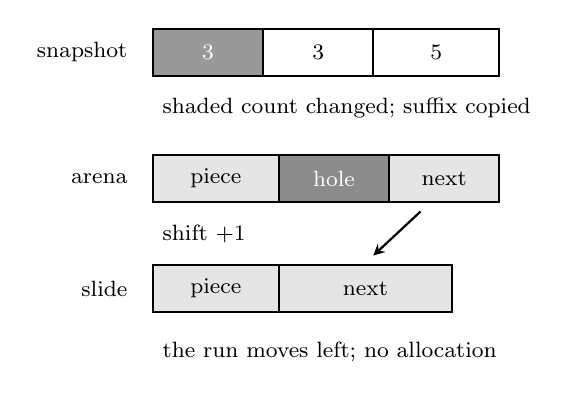
\begin{tikzpicture}[x=1mm, y=1mm, font=\footnotesize]
  \node[anchor=east] at (16,32) {snapshot};
  \draw[thick, fill=black!40] (18,29) rectangle (32,35);
  \node[text=white] at (25,32) {3};
  \draw[thick, fill=white] (32,29) rectangle (46,35);
  \node at (39,32) {3};
  \draw[thick, fill=white] (46,29) rectangle (62,35);
  \node at (54,32) {5};
  \node[anchor=west] at (18,25) {shaded count changed; suffix copied};

  \node[anchor=east] at (16,16) {arena};
  \draw[thick, fill=black!10] (18,13) rectangle (34,19);
  \node at (26,16) {piece};
  \draw[thick, fill=black!45] (34,13) rectangle (48,19);
  \node[text=white] at (41,16) {hole};
  \draw[thick, fill=black!10] (48,13) rectangle (62,19);
  \node at (55,16) {next};
  \node[anchor=west] at (18,9) {shift $+1$};
  \draw[-stealth, thick] (52,11.8) -- (46,6.2);

  \node[anchor=east] at (16,2) {slide};
  \draw[thick, fill=black!10] (18,-1) rectangle (34,5);
  \node at (26,2) {piece};
  \draw[thick, fill=black!10] (34,-1) rectangle (56,5);
  \node at (45,2) {next};
  \node[anchor=west] at (18,-6) {the run moves left; no allocation};
\end{tikzpicture}
\caption{Delete of one key in the first piece, whose relative count goes from 4 to 3.
The snapshot copies the suffix from the next old start.
In the arena the following piece is one slot to the right, so its shift is $+1$, and a lookup adds that shift to the rank.
The bottom row slides that piece into the hole.
A planted insert spare is a larger hole of the same kind, and this slide does not remove it.}
\label{fig:arch}
\end{figure}

\begin{algorithm}[t]
\caption{Local re-fit after one insert or delete.}
\label{alg:refit}
\begin{algorithmic}[1]
\STATE Move the key inside its anchor piece, merging or splitting that piece on the anchor rule
\STATE Find the segment $s$ whose start key is the rightmost start $\le$ the edited key
\STATE Restart at segment $s-1$ (or at $0$)
\STATE Emit new segments until the origin the fitter would open next equals an old start strictly after the edit, or the array ends
\STATE Splice those segments in and keep the untouched suffix
\STATE Add the rank change to later prefix blocks
\STATE If a leaf start key changed, splice the upper models up to the first unchanged leaf boundary
\end{algorithmic}
\end{algorithm}

The restart at $s-1$ is required because the edited key may have been what stopped the previous piece.
The stop rule copies the suffix only when that next origin is an old start.
A count-cap split or an appearing anchor is the same test: they change where the next origin is.

\textbf{Theorem 1.}
Fix $\varepsilon$, $M$, and a streaming segmenter that starts each segment at the cursor and whose fields depend only on the keys from that cursor, $\varepsilon$, the 65{,}535-key cap, and the anchor predicate.
The secret is not in $\mathrm{Repr}$. Prefix sums are a cache and are not serialized.
The cursor emits a new segment only from a key the edit has not passed.
It copies the stored suffix only when that key equals an old start key.
A level that is empty, or no longer shorter than the keys it models, is replaced by the same \texttt{Build} the constructor uses.
Under that invariant, Algorithm~\ref{alg:refit} emits the same segment sequence as \texttt{Build} on the updated array, so $\mathrm{Repr}$ is strongly history independent for one binary.

\textbf{Proof.}
The proof has four parts.

\emph{Canonicity.}
The segmenter is a deterministic function of the sorted keys from its cursor, $\varepsilon$, the 65{,}535-key cap, and the anchor predicate $\mathrm{splitmix64}(x+s)\bmod M=0$ with $s$ fixed.
\texttt{Build} therefore emits one segment sequence for a given set.
Two update sequences that arrive at the same set have the same \texttt{Build} image.
It remains to show that the local edit produces that image.

\emph{Prefix invariance.}
Let the edited key fall in segment $s$, and let the restart index be the start of segment $s-1$, or the start of the array when $s=0$.
Every segment that ended at or before that index was fitted on a prefix the edit does not change, so those stored fields stay.
Restarting one segment early is required for deletion: the deleted key may have been the point that closed segment $s-1$, and the same fitter on the surviving prefix may now extend it.

\emph{Resynchronization.}
From the restart index the algorithm calls the same segmenter as \texttt{Build}, on the same remaining keys.
It copies the stored suffix if and only if the origin that fitter is about to open equals an old start key strictly after the edit.
That origin is a \texttt{Build} origin because the test runs at a fitter cursor, the restart key is prefix-invariant, and each segment depends only on keys from its cursor.
Relative counts do not depend on the number of keys before the cursor, so the stored suffix matches byte for byte.
If no such origin exists, the algorithm runs to the end of the array, which is exactly what \texttt{Build} does from the restart index.

\emph{Upper levels and induction.}
The upper model is the same segmenter applied to the leaf start keys, with the same anchor predicate.
If the splice leaves every leaf start key unchanged, the upper tables stay and only the stored fields of the edited segments change.
If a start key changes, the same resynchronization is applied to the leaf start keys, and the copy is taken only when that origin is also at or after the first unchanged leaf start.
That splice writes the existing slots when the new span has the same length, and it replaces the level vector when the length changes.
If the level is then empty, or no longer shorter than the keys it models, the whole hierarchy is rebuilt.
The resulting upper tables are the ones \texttt{Build} would have stored.
Prefix sums are a cache. A delete adds one constant to every later prefix, and that constant is stored once per block of segments rather than written into every segment.
By induction on the update sequence, every reachable state has the bytes of \texttt{Build} on its current key set.

The fuzzer drew one million inserts and deletes from a 2{,}048-key universe and compared both the optimal hull and the greedy shrinking cone~\cite{galakatos2019fiting}, and a hash-promotion tree, to a fresh build every 250 operations.
All 4{,}000 comparisons matched on Apple Clang, including lookups after inserts on the signed-shift arena, with a compaction limit of 4.
GCC 13.3 matched the same 4{,}000/4{,}000 checks, including the signed shift and that limit, in 17.3\,s.
Mean re-fit on that GCC run was 2.19 segments for the optimal hull and 2.16 for the greedy cone.
The SOSD byte checks in Section~\ref{sec:eval} are GCC on the signed-shift layout.
A 4{,}096-key quadratic set, after one delete, produced the same 2{,}569 snapshot bytes on Apple Clang and on GCC 13.3.
That is one input.
A slope computed with fused multiply-add on one machine can still differ in the last bit from the other.
$\mathrm{Repr}$ is defined for one binary.

\subsection{Bytes in a snapshot}

A serialized snapshot begins with the four bytes \texttt{SHI2}, then the error bound, the anchor modulus, the segmenter identity, and the level count.
Each level is a count followed by its segments.
One segment is 16 bytes: the first key as \texttt{uint64}, the slope as \texttt{float} with a zero slope stored as $+0$, the intercept as \texttt{int16}, and the key count as \texttt{uint16}.
The secret, the key array, and the prefix sums used at lookup are absent.
The comparison that the fuzzer and the SOSD harness call byte-identical is this buffer against the buffer of a fresh \texttt{Build} in the same process.

The stored start key is a key of the current set.
Fig.~\ref{fig:layout} is the record that holds it.
On an index of user identifiers, email hashes, or cell ids, that field is the identifier itself.
Erasure of the key from the table therefore has to remove it from this field as well, which is what the splice does: a start key that belonged only to the deleted key cannot survive into \texttt{Build} of the survivors, and the theorem says the splice matches that build.

\subsection{Cascade length}

Without anchors, the keys $K[i]=i^{2}$ have no reason to put a new boundary back on an old one.
One deletion can shift every later segment.
On 200{,}000 such keys a delete rewrote a mean of 21 of 56 segments.
With $M=4096$ the maximum in that sample was 7.
The expected gap between anchors is about $M$ keys when the hash is balanced, so the recomputed region is a few segments in expectation.
Fig.~\ref{fig:cascade} is that geometry.
The bound is an expectation under the hash, and it is an envelope rather than the typical SOSD case.
If the fitter does not resynchronize on an old start key, the walk ends at the next anchor.
Under a balanced keyed hash each key is an anchor with probability $1/M$, independently of the others, so the number of keys until the next anchor is geometric:
$\mathrm{P}[\mathrm{walk}>tM]=(1-1/M)^{tM}\le e^{-t}$.
That is the $i^{2}$ walk.
A streaming fitter that refuses to resynchronize rewrites every segment until that anchor, which is $O(M)$ keys and $O(M/L+1)$ segments when the mean segment holds $L$ keys.
The squared-key sample rewrote at most 7 segments.
The 512-draw maximum on the SOSD files is 14 segments.
Those files hold fewer keys per segment than the squared keys, so the same anchor gap covers more segments, and a draw of 512 positions sees a higher maximum than a draw of a few deletes.
An exposed secret is the availability issue stated with the anchor rule, and only the length of this walk depends on it.

On the SOSD files the fitter resynchronizes earlier than the next anchor.
Wiki at $M=4096$ holds about $1{,}350$ keys per segment, so an anchor gap covers about three segments, and the measured mean re-fit is $2.5$.
Fb holds about $89$ keys per segment, so the same modulus covers on the order of $46$ segments, while the measured mean re-fit is $2.25$.
The stop rule is the next old start key, and on these distributions that start key reappears within a few segments.
Anchors are the cap for the family that never puts an old start key back.
They are optional on a distribution whose unanchored re-fit is already a handful of segments, which is what $M=0$ shows for wiki, fb, and books.

On the real SOSD files the cascade is shorter than the convex lower bound, and it does not require a small $M$.
Table~\ref{tab:anchor} and the right panel of Fig.~\ref{fig:cost} vary $M$ on the full wiki, fb, and books files.
Four deletes at every modulus, including $M=0$, matched a rebuild.
Mean re-fit stayed between 2.25 and 4 segments.
On wiki, $M=4096$ is $2.37\times$ static PGM with mean re-fit $2.50$ and a $0.63$\,ms mean delete, and $M=0$ is $1.12\times$ with mean re-fit $3.00$ and a $24.8$\,ms mean delete, because the piece is the file.
The same file at $M=1024$ is $6.31\times$, and its levels are $119{,}803$, $88{,}723$, and $88{,}722$ segments.
At $M=4096$ they are $67{,}065$, $22{,}273$, and $22{,}261$.
The last of those levels has about $n/M$ segments and does not shrink, because the upper model uses the same anchor rule and an anchor start is an anchor again.
Extra leaves over static PGM, divided by $n/M$, are about $0.9$ on wiki, $2.8$ on fb, $2.2$ on books, and $2.6$ on osm.
Static PGM on wiki is $46{,}818$, $269$, $4$, and $1$ segments, $753{,}576$ bytes in all.
On fb and books, $M=4096$ costs $1.10\times$ and $1.28\times$.
Dropping the anchors moves the mean re-fit from 2.25 to 3.00 on fb and from 3.50 to 3.75 on books.
The convex family is why the mechanism exists.
On the SOSD files a deployment can choose a large $M$, or none, once the cascade has been measured.

\begin{figure}[t]
\centering
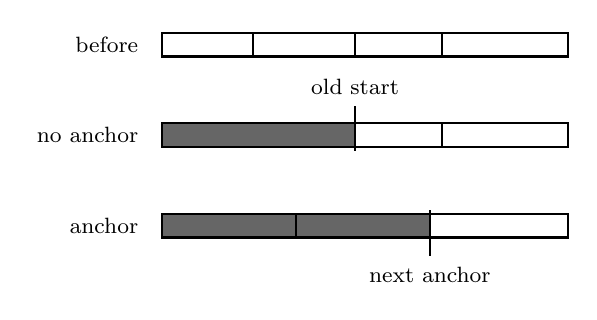
\begin{tikzpicture}[font=\footnotesize,
  seg/.style={draw, thick, minimum height=12pt, inner sep=0pt}]
\node[anchor=east] at (-0.18,2.20) {before};
\draw[seg, fill=white] (0,2.05) rectangle (1.15,2.35);
\draw[seg, fill=white] (1.15,2.05) rectangle (2.45,2.35);
\draw[seg, fill=white] (2.45,2.05) rectangle (3.55,2.35);
\draw[seg, fill=white] (3.55,2.05) rectangle (5.15,2.35);

\node[anchor=east] at (-0.18,1.05) {no anchor};
\draw[seg, fill=black!60] (0,0.90) rectangle (2.45,1.20);
\draw[thick] (2.45,0.85) -- (2.45,1.42);
\node[anchor=south] at (2.45,1.44) {old start};
\draw[seg, fill=white] (2.45,0.90) rectangle (3.55,1.20);
\draw[seg, fill=white] (3.55,0.90) rectangle (5.15,1.20);

\node[anchor=east] at (-0.18,-0.10) {anchor};
\draw[seg, fill=black!60] (0,-0.25) rectangle (1.7,0.05);
\draw[seg, fill=black!60] (1.7,-0.25) rectangle (3.4,0.05);
\draw[thick] (3.4,-0.48) -- (3.4,0.10);
\node[anchor=north] at (3.4,-0.50) {next anchor};
\draw[seg, fill=white] (3.4,-0.25) rectangle (5.15,0.05);
\end{tikzpicture}
\caption{Where a local re-fit stops.
The middle row is the SOSD case: an old start key reappears, and the white suffix is copied.
The bottom row is the case with no such key, as on $i^{2}$.
The re-fit then runs to the next anchor.}
\label{fig:cascade}
\end{figure}

\begin{figure}[t]
\centering
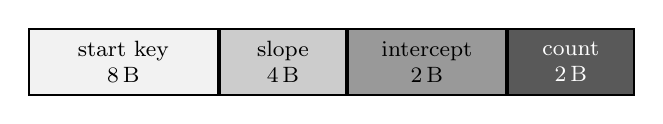
\begin{tikzpicture}[font=\footnotesize, cell/.style={draw, thick, minimum height=18pt, inner sep=1pt, anchor=west, align=center}]
\node[cell, fill=black!5, minimum width=24mm, text width=22mm, minimum height=24pt] (k) at (0,0) {start key\\8\,B};
\node[cell, fill=black!20, minimum width=16mm, text width=14mm, minimum height=24pt, right=0pt of k] (s) {slope\\4\,B};
\node[cell, fill=black!40, minimum width=20mm, text width=18mm, minimum height=24pt, right=0pt of s] (i) {intercept\\2\,B};
\node[cell, fill=black!65, minimum width=16mm, text width=14mm, minimum height=24pt, text=white, right=0pt of i] (c) {count\\2\,B};
\end{tikzpicture}
\caption{One segment in the serialized snapshot, 16 bytes.
The intercept and the count are local to the segment.
The anchor secret and the key array are not in this record.}
\label{fig:layout}
\end{figure}

\section{Erasure latency}
\label{sec:latency}

Erasure latency is the time from the request until a published snapshot no longer contains the key.
A full static fit is one way to get there.
On these files that fit is neither free nor the 0.3\,s figure that a quiet microbenchmark of PGM can suggest.
On the shared Xeon host of Section~\ref{sec:eval}, a static PGM build took 2.30\,s for the 90.4 million distinct wiki keys, 7.58\,s for fb, 6.14\,s for books, and 28.9\,s for osm.
A fresh build of the arena index, in the same run as the 512-delete sample, took 3.98\,s, 27.7\,s, 14.7\,s, and 101\,s.
An earlier prefix of the first 10 million wiki records, 8.84 million distinct keys, took 277\,ms for PGM and 516\,ms for this index.
Table~\ref{tab:build} is the full-file construction time on the same inputs as the delete measurements.

\begin{table}[t]
\caption{One-shot construction on the Xeon.
The PGM column is a separate run on the same files.
The other column is one fresh build of the arena index in the 512-delete run.
Each delete in that run copies the index and keeps the spare capacity of the built arena.
This is the cost of erasing the key by throwing the old model away.}
\label{tab:build}
\centering
\footnotesize
\begin{tabular}{@{}lrr@{}}
\toprule
File & This index & Static PGM \\
\midrule
wiki  & 3.98\,s & 2.30\,s \\
fb    & 27.7\,s & 7.58\,s \\
books & 14.7\,s & 6.14\,s \\
osm   & 101\,s & 28.9\,s \\
\bottomrule
\end{tabular}
\end{table}

Batching deletes into that rebuild leaves the old model published until the batch is installed.
A rebuild once a minute leaves the deleted key in the index for up to a minute, and rebuilding on every delete makes the wait the full fit, which reads every surviving key.
Dynamic PGM returns immediately and adds 16 bytes that still hold the key, so the time until the call returns and the time until the key is gone from the published model are different quantities.

The delete timed below removes the key from its anchor piece and then runs Algorithm~\ref{alg:refit}.
Both steps are inside the timer.
Table~\ref{tab:e2e} is an earlier measurement on a single contiguous array at 200{,}000 keys, where the array move was 12--15\,$\mu$s and the re-fit was 36--48\,$\mu$s.
Table~\ref{tab:sosd} is that same contiguous layout on the SOSD files, on a handful of probes, with the full-array move separated from the model re-fit.
A later 512-position sample of that layout had means of 33\,ms, 149\,ms, 103\,ms, and 535\,ms.
Those times are the linear slide of the whole key array.
Table~\ref{tab:dist} replaces them.
The keys are cut on the anchors, the upper models are spliced instead of rebuilt, and a rank change is added to later prefix blocks.

A packed-memory array would give a logarithmic move with density thresholds~\cite{bender2016}.
We cut the array at the anchors the model already uses, so Table~\ref{tab:modtime} times a linear piece move: 24.2\,ms to 215\,ms at $M=0$, and 2.3\,$\mu$s to 3.8\,$\mu$s at $M=4096$.
This paper does not implement that PMA.
The hash-promotion tree used in the fuzzer is history independent because every level is a function of the key set, and its insert and erase rebuild those levels.
It is a second exact object for the byte check.
Its lookup cost is reported below, and its update cost is the cost of that rebuild.
We do not use it as evidence that a history-independent B-tree is slower than this index.

\section{Evaluation}
\label{sec:eval}

\subsection{Setup}

Two machines appear in the tables.
The 200{,}000-key rows and one fuzzer run used Apple Silicon and Apple Clang at \texttt{-O3}.
The SOSD rows, the lookup rows, the anchor sweep, and the second fuzzer run used a Dell R760 with an Intel Xeon Gold 6430, 64 threads, 251\,GB of RAM, GCC 13.3 at \texttt{-O3}, one thread.
That host was shared, so absolute times are a loaded-server measurement.
Lookup ratios and the byte comparisons ran in one process.
The static PGM column of Table~\ref{tab:build} is a separate run on the same files, and the 813, 125, 325, and 156 figures divide that run by the slowest deletes in Table~\ref{tab:dist}.
The Mean/Max $\times$ column of Table~\ref{tab:dist} divides the same-run rebuild of this index, not that static PGM column.
The timed \texttt{erase} is the piece move, the local fit, and the boundary-list rebuild. The copy and the leaf start-key array are taken before the clock. The run slide is off in that table. Dynamic PGM and ALEX erase are not timed, because those calls retain the key. A packed-memory array was not implemented.

Unless a table says otherwise, $\varepsilon=16$, the recursive error is $4$, the anchor modulus is $4096$, the segmenter is the optimal hull, and the anchor secret is fixed.
SOSD binaries are the Zenodo release 15240501.
Each file is a count header followed by keys.
We sort and drop duplicates.
Books is stored as \texttt{uint32} and widened to \texttt{uint64}.
Wiki yields 90{,}437{,}011 distinct keys from the 200-million-record file.
Fb and osm are already distinct at 200 million and 800 million keys.
Books drops one duplicate from 200 million.
The 200{,}000-key rows are generators with the shape of those distributions, not prefixes of the binaries.
They are labeled as generators wherever they appear.

\subsection{End-to-end deletion}

\begin{table}[t]
\caption{End-to-end delete on 200{,}000-key generators (Apple Clang), on one contiguous key array.
The timer includes the array move and the re-fit.
Every lookup was exact.
Every one of 20 deletes matched a rebuild.
Dynamic PGM grew by 16 bytes per erase, and the tombstone was present, on all four sets.}
\label{tab:e2e}
\centering
\footnotesize
\begin{tabular}{@{}lrrrrr@{}}
\toprule
Set & Segs & Misses & Delete & Rebuild & $\times$ \\
\midrule
books & 182 & 0 & 60\,$\mu$s & 1.88\,ms & 31 \\
fb    & 2{,}596 & 0 & 49\,$\mu$s & 2.95\,ms & 60 \\
osm   & 733 & 0 & 53\,$\mu$s & 2.37\,ms & 45 \\
wiki  & 340 & 0 & 48\,$\mu$s & 2.04\,ms & 42.5 \\
\bottomrule
\end{tabular}
\end{table}

\begin{table}[t]
\caption{Contiguous key array, before the keys were cut into anchor pieces.
Each cell is the mean of 8 deletes on wiki, fb, and books, and of 4 deletes on osm.
The delete column moves a suffix and rebuilds the upper levels.
Table~\ref{tab:dist} is the later piece store, and its rebuild column is not this one.}
\label{tab:sosd}
\centering
\footnotesize
\begin{tabular}{@{}lrrrrrr@{}}
\toprule
File & Keys & Move & Model & Delete & Rebuild & $\times$ \\
\midrule
wiki  & 90.4M & 31.8\,ms & 4.64\,ms & 36.4\,ms & 3.01\,s & 83 \\
fb    & 200M  & 73.4\,ms & 39.6\,ms & 113\,ms & 8.59\,s & 76 \\
books & 200M  & 68.8\,ms & 42.2\,ms & 111\,ms & 7.27\,s & 65 \\
osm   & 800M  & 216\,ms & 138\,ms & 354\,ms & 33.0\,s & 93 \\
\bottomrule
\end{tabular}
\end{table}

\begin{table}[t]
\caption{End-to-end delete over 512 uniform ranks on the Xeon, with no boundary slide and the vacated tail cleared.
Each trial copies a built index and times one \texttt{erase}.
The copy and the leaf start keys are taken before the clock.
Rebuild is a fresh build of this index in the same run.
Mean\,/\,max divides the rebuild in the row by the mean and by the maximum in the row.}
\label{tab:dist}
\centering
\scriptsize
\begin{tabular}{@{}lrrrrrrr@{}}
\toprule
File & Mean & Std & P50 & P99 & Max & Rebuild & Mean\,/\,Max\,$\times$ \\
\midrule
wiki  & 0.67\,ms & 0.40 & 0.53 & 2.46 & 2.83 & 3.98\,s & 5{,}940\,/\,1{,}406 \\
fb    & 2.20\,ms & 6.18 & 1.33 & 31.8 & 60.7 & 27.7\,s & 12{,}591\,/\,456 \\
books & 1.47\,ms & 2.75 & 1.36 & 18.7 & 18.9 & 14.7\,s & 10{,}000\,/\,778 \\
osm   & 7.61\,ms & 19.5 & 1.14 & 99.1 & 185 & 101\,s & 13{,}272\,/\,546 \\
\bottomrule
\end{tabular}
\end{table}

Table~\ref{tab:e2e} is the cache-resident pilot on the contiguous array.
Mean re-fit length was 2.6--3.2 segments (maximum 5--7).
Model-only time was 36--48\,$\mu$s.
Table~\ref{tab:sosd} is the mean of that layout: 8 deletes on wiki, fb, and books, and 4 on osm.
The audits on that layout covered 90{,}437{,}011, 200{,}000{,}000, 199{,}999{,}999, and 800{,}000{,}000 keys, and missed none.
Table~\ref{tab:dist} is the arena.
One hundred further uniform ranks on each file, each compared with a fresh build of the survivors, matched on all 400 trials.
The packed binary matched on 8 further deletes of each file.
Mean re-fit on those checks was 2.77, 2.63, 3.08, and 2.70 segments (maximum 6, 7, 9, and 13).
Mean re-fit on the 512-draw is 2.70, 2.77, 3.08, and 2.83 segments (maximum 9, 8, 14, and 14).
The sample is two clusters.
The slow one changes a leaf start key and splices the upper models.
The piece move is a few microseconds in both clusters at this modulus, which the repeat below separates from the refit.
On osm the median is 1.14\,ms and the mean is 7.61\,ms, so more than half of the draws are in the fast cluster and the mean is the slow one.
On books the median, 1.36\,ms, sits close to the mean, 1.47\,ms.
On wiki the 99th percentile is 2.46\,ms and the maximum is 2.83\,ms, against the 3.98\,s build in that run.
The slowest delete finishes $1{,}406\times$, $456\times$, $778\times$, and $546\times$ sooner than a fresh build of the arena index in the same run, whose times are the ``This index'' column of Table~\ref{tab:build}.
On an earlier binary, a batch of 32 deletes on one copy took 0.47\,ms, 2.80\,ms, 1.57\,ms, and 25.7\,ms per delete and matched a fresh build of the survivors on all four files.
That batch is one sequence of 32 erases, not 32 copies of the single-delete tail.
The final model of the 20{,}000-operation mix matched a fresh build on all four files as well.
The 100 single-delete checks are a separate comparison.
The mean rate is about 1{,}500 deletes per second on wiki, 455 on fb, 680 on books, and 131 on osm.

\subsection{Space and lookup}

\begin{table}[t]
\caption{Model size on the SOSD files at $\varepsilon=16$ and $M=4096$.
Both sizes include upper levels.
The segment counts are the leaf level.
Levels counts this index only.
Wiki is $1{,}785{,}584/753{,}576=2.37\times$; the megabyte cells are rounded.}
\label{tab:space}
\centering
\footnotesize
\begin{tabular}{@{}lrrrrr@{}}
\toprule
File & SHI segs & PGM segs & SHI & PGM & Levels \\
\midrule
wiki  & 67{,}065 & 46{,}818 & 1.79\,MB & 0.75\,MB & 3 \\
fb    & 2{,}255{,}847 & 2{,}120{,}485 & 38.6\,MB & 35.0\,MB & 3 \\
books & 837{,}007 & 729{,}231 & 15.0\,MB & 11.7\,MB & 3 \\
osm   & 6{,}690{,}022 & 6{,}175{,}387 & 118\,MB & 101\,MB & 4 \\
\bottomrule
\end{tabular}
\end{table}

Those sizes are the serialized model, leaves and upper levels together.
The two wiki upper levels at $M=4096$, $22{,}273$ and $22{,}261$ segments, are $712{,}544$ bytes, $0.71$\,MB.
On fb, books, and osm the same modulus ends in a level of about $n/M$ segments as well: $49{,}268$, $48{,}606$, and $195{,}281$.
The key arena stores the live keys and reserves capacity for $4n+65536$ keys, so a merge does not reallocate inside the delete timer.
The factor of four is spare capacity kept on a copy of the index: without it, the first slot allocation after that copy reallocates the arena inside the timer.
The reservation is virtual address space.
On osm it is about 25\,GB for 6.4\,GB of live keys.
The PGM column is that full model, not the leaf table alone.
On wiki the bytes above the leaf table are $753{,}576-46{,}818\times 16=4{,}488$.
The four named levels are $47{,}092$ segments, $753{,}472$ bytes.
The remaining $104$ bytes are four sentinel segments and the level-offset array.
At $M=4096$, fb, books, and osm are between $1.10\times$ and $1.28\times$ static PGM, and wiki is $2.37\times$.
That $2.37\times$ is $1{,}785{,}584/753{,}576$.
The table's megabyte cells are rounded; the $2.37\times$ figure uses the exact bytes in the caption of Table~\ref{tab:space}.
Table~\ref{tab:anchor} shows that the wiki overrun is the anchor density: with $M=0$ the same file is $1.12\times$.
Those sizes keep upper-level anchors on.
Turning that rule off leaves the leaf anchors and the piece cuts, and the upper levels are an ordinary recursive fit.
The model is then $1{,}082{,}144$ bytes on wiki, $37{,}357{,}600$ on fb, $13{,}449{,}520$ on books, and $110{,}111{,}648$ on osm, which is $1.44\times$, $1.07\times$, $1.15\times$, and $1.09\times$ static PGM.
Leaf counts stay $67{,}065$, $2{,}255{,}847$, $837{,}007$, and $6{,}690{,}022$.
Eight deletes on each file matched a fresh build of that variant and averaged 0.60\,ms, 9.98\,ms, 2.07\,ms, and 31.8\,ms, with upper splice 0.18\,ms, 9.52\,ms, 1.64\,ms, and 30.6\,ms, a different draw from Table~\ref{tab:modtime}.
The tables in this paper keep the upper anchors on, and they keep a level that is shorter than the level below it.
A variant that instead drops a level unless it is shorter than half the level below it, still at $M=4096$, is $1{,}429{,}408$ bytes on wiki, $38{,}604{,}336$ on fb, $14{,}173{,}088$ on books, and $112{,}091{,}360$ on osm: $1.90\times$, $1.10\times$, $1.21\times$, and $1.10\times$ static PGM.
Wiki, books, and osm drop the last $n/M$ level; fb keeps it.
Eight deletes of that variant, with the vacated tail cleared, matched a fresh build on $\mathrm{Repr}$ and on the packed rank-order keys on every file, and averaged 0.49\,ms, 1.67\,ms, 0.61\,ms, and 3.83\,ms.
The published tables do not use that rule.
The dashed line in the right panel of Fig.~\ref{fig:cost} is $1.5\times$ static PGM, a reference line for that wiki point.
Table~\ref{tab:lookup} and the left panel of Fig.~\ref{fig:cost} are one million queries on a fresh arena, drawn from the key set, with no preceding scan of the keys.
This index is $1.68$--$2.00\times$ static PGM: 390\,ns, 588\,ns, 506\,ns, and 743\,ns against 219\,ns, 294\,ns, 261\,ns, and 441\,ns.
The hash-promotion tree took 545\,ns, 641\,ns, 645\,ns, and 821\,ns in the same runs.
That tree is rebuilt on every update, so staying under it is not an update-cost comparison.
The fresh arena is in that neighborhood because the keys are rank-contiguous and the piece directory is not consulted.
After one delete the same million probes, timed with the tree on the same keys, took 395\,ns, 595\,ns, 508\,ns, and 748\,ns, against 554\,ns, 656\,ns, 653\,ns, and 837\,ns.
All four stay under the tree, and none of the probes missed.
After 1{,}024 further deletes the times are 465\,ns, 662\,ns, 587\,ns, and 821\,ns, against 554\,ns, 652\,ns, 653\,ns, and 838\,ns.
Wiki, books, and osm stay under the tree.
Fb does not.
A separate exhaustive lookup, after a different draw of 1{,}024 uniform deletes, missed none of the survivors on any file.
Section~\ref{sec:compact} is a later run that slides one run of pieces once the boundary list passes 32 entries, which puts fb back under the tree.
The hash-promotion tree stores 70\,MB, 155\,MB, 155\,MB, and 619\,MB of node keys, because each level keeps the promoted keys.
That tree is rebuilt on every update.
It is the history-independent control for bytes and for lookup, and it is not a packed-memory array.

\begin{table}[t]
\caption{Lookup on the Xeon, mean of one million queries drawn from the key set, on a fresh arena.
PGM time includes the final binary search of its error window.
The tree column is the hash-promotion history-independent tree in the same run.
ALEX is a separate million-query run on the same files.
It is not the paired tree run.}
\label{tab:lookup}
\centering
\footnotesize
\begin{tabular}{@{}lrrrr@{}}
\toprule
File & PGM & SHI & HI tree & ALEX \\
\midrule
wiki  & 219\,ns & 390\,ns & 545\,ns & 79\,ns \\
fb    & 294\,ns & 588\,ns & 641\,ns & 604\,ns \\
books & 261\,ns & 506\,ns & 645\,ns & 149\,ns \\
osm   & 441\,ns & 743\,ns & 821\,ns & 891\,ns \\
\bottomrule
\end{tabular}
\end{table}

\begin{figure*}[t]
\centering
\begin{minipage}[t]{0.48\textwidth}
\centering
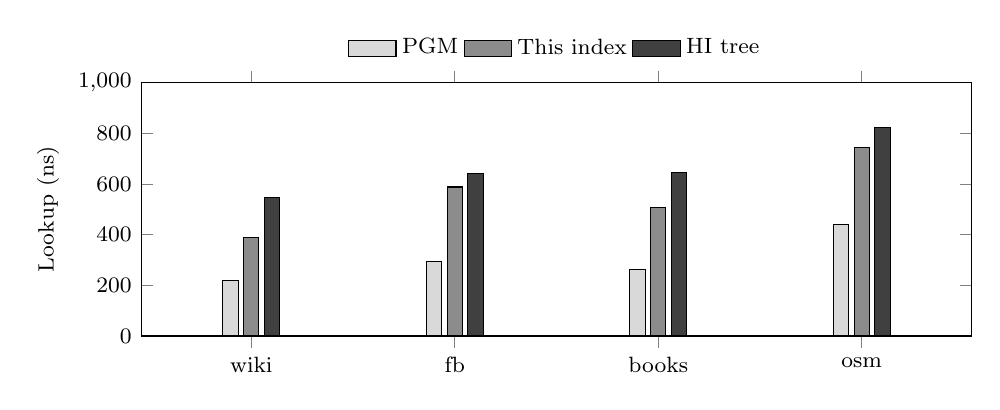
\begin{tikzpicture}
\begin{axis}[
    ybar,
    area legend,
    bar width=5.5pt,
    width=\textwidth,
    height=4.8cm,
    ymin=0, ymax=1000,
    ylabel={Lookup (ns)},
    symbolic x coords={wiki, fb, books, osm},
    xtick=data,
    enlarge x limits=0.18,
    legend style={at={(0.5,1.05)}, anchor=south, legend columns=3, font=\footnotesize, draw=none, inner sep=2pt, cells={anchor=west}},
    every axis plot/.append style={draw=black, thin},
    tick label style={font=\footnotesize},
    label style={font=\footnotesize},
]
\addplot[fill=black!15] coordinates {(wiki,219) (fb,294) (books,261) (osm,441)};
\addplot[fill=black!45] coordinates {(wiki,390) (fb,588) (books,506) (osm,743)};
\addplot[fill=black!75] coordinates {(wiki,545) (fb,641) (books,645) (osm,821)};
\legend{PGM, This index, HI tree}
\end{axis}
\end{tikzpicture}
\end{minipage}\hfill
\begin{minipage}[t]{0.48\textwidth}
\centering
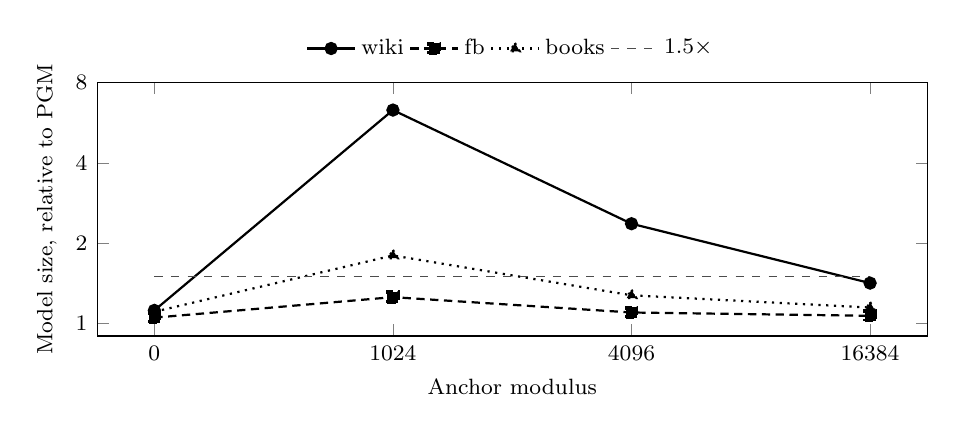
\begin{tikzpicture}
\begin{axis}[
    width=\textwidth,
    height=4.8cm,
    ymin=0.9, ymax=8,
    ymode=log,
    log origin=infty,
    log ticks with fixed point,
    ytick={1,2,4,8},
    ylabel={Model size, relative to PGM},
    symbolic x coords={0, 1024, 4096, 16384},
    xtick=data,
    xlabel={Anchor modulus},
    enlarge x limits=0.08,
    legend style={at={(0.5,1.05)}, anchor=south, legend columns=4, font=\footnotesize, draw=none, inner sep=2pt, cells={anchor=west}},
    tick label style={font=\footnotesize},
    label style={font=\footnotesize},
]
\addplot[black, mark=*, thick] coordinates {(0,1.122) (1024,6.311) (4096,2.369) (16384,1.420)};
\addplot[black, mark=square*, densely dashed, thick] coordinates {(0,1.054) (1024,1.258) (4096,1.102) (16384,1.071)};
\addplot[black, mark=triangle*, dotted, thick] coordinates {(0,1.109) (1024,1.802) (4096,1.278) (16384,1.150)};
\addplot[black!70, dashed, line legend] coordinates {(0,1.5) (1024,1.5) (4096,1.5) (16384,1.5)};
\legend{wiki, fb, books, $1.5\times$}
\end{axis}
\end{tikzpicture}
\end{minipage}
\caption{Left: lookup on a fresh arena, against static PGM and the hash-promotion tree.
Right: model size relative to static PGM as the anchor modulus changes, on a logarithmic vertical axis.
$M=0$ is an unanchored fit.
The dashed line is $1.5\times$ static PGM, drawn as a reference.}
\label{fig:cost}
\end{figure*}

\begin{table}[t]
\caption{Anchor modulus on the full SOSD files.
Space is the model size over static PGM.
Each modulus had four deletes, all byte-identical to a rebuild.
Refit is the mean number of segments rewritten.}
\label{tab:anchor}
\centering
\footnotesize
\begin{tabular}{@{}llrrr@{}}
\toprule
File & $M$ & Space & Refit & Max \\
\midrule
wiki  & 0     & 1.12$\times$ & 3.00 & 3 \\
wiki  & 1024  & 6.31$\times$ & 2.75 & 3 \\
wiki  & 4096  & 2.37$\times$ & 2.50 & 3 \\
wiki  & 16384 & 1.42$\times$ & 4.00 & 5 \\
\addlinespace
fb    & 0     & 1.05$\times$ & 3.00 & 4 \\
fb    & 1024  & 1.26$\times$ & 2.75 & 4 \\
fb    & 4096  & 1.10$\times$ & 2.25 & 3 \\
fb    & 16384 & 1.07$\times$ & 2.25 & 3 \\
\addlinespace
books & 0     & 1.11$\times$ & 3.75 & 6 \\
books & 1024  & 1.80$\times$ & 2.25 & 3 \\
books & 4096  & 1.28$\times$ & 3.50 & 6 \\
books & 16384 & 1.15$\times$ & 3.25 & 5 \\
\bottomrule
\end{tabular}
\end{table}

\subsection{Compacting the boundary list}
\label{sec:compact}

Each delete adds a boundary, and the lookup binary-searches that list.
Pieces that share a shift already sit in one contiguous run, and the boundary is a hole in front of that run.
When the list exceeds 32 entries, the index slides the smallest run whose hole contains no other live piece left into that hole, then subtracts the hole from the run's offsets.
The slide does not allocate.
A slide that would overlap another live piece is skipped, so 32 is a target rather than a hard ceiling.
Copying every live key into a fresh rank-ordered buffer, the policy this slide replaces, paused for 0.41\,s, 0.90\,s, 0.90\,s, and 3.6\,s.
The slide does not change the serialized model: the million-operation fuzzer, run on Apple Clang with a limit of 4, still matched a fresh build on all 4{,}000 checks.
Every probe in Table~\ref{tab:compact} missed none.
After 4{,}096 deletes the list length is 32 on every file.
The slide ran 4{,}053, 4{,}058, 4{,}054, and 4{,}062 times.

\begin{table}[t]
\caption{Point lookup after deletes with the run slide, this index over the history-independent tree, in nanoseconds.
One million probes in the same process, paired with the tree in that run.
The limit is 32 boundaries.
Worst is the slowest slide in the 4{,}096 deletes.
Amortized divides the total slide time by 4{,}096.
Table~\ref{tab:dist} does not include these slides: its limit is zero.}
\label{tab:compact}
\centering
\scriptsize
\begin{tabular}{@{}lrrrr@{}}
\toprule
File & 1 delete & 4{,}096 & Worst slide & Amortized \\
\midrule
wiki  & 395\,/\,527 & 420\,/\,527 & 1.18\,ms & 0.43\,ms \\
fb    & 517\,/\,621 & 551\,/\,626 & 3.72\,ms & 1.00\,ms \\
books & 445\,/\,619 & 475\,/\,621 & 2.68\,ms & 1.02\,ms \\
osm   & 683\,/\,789 & 770\,/\,815 & 10.7\,ms & 4.03\,ms \\
\bottomrule
\end{tabular}
\end{table}

All four stay under the tree after 4{,}096 deletes.
The slowest slide is 1.18\,ms, 3.72\,ms, 2.68\,ms, and 10.7\,ms.
Against the ``This index'' builds in Table~\ref{tab:build} the slowest slide is 3{,}373$\times$, 7{,}446$\times$, 5{,}485$\times$, and 9{,}439$\times$.
Spread across the 4{,}096 deletes, the slide is 0.43\,ms, 1.00\,ms, 1.02\,ms, and 4.03\,ms per delete.
On fb the same limit was continued to 100{,}001 deletes.
Lookup was then 612\,ns against the tree at 643\,ns, with no missed probes.
The list had 38 entries, 99{,}860 slides had run, and those slides totaled 292\,s.
That is 2.92\,ms per delete.
The slowest slide in that run was 16\,ms.
Fig.~\ref{fig:slide} is the lookup ratio at each step of the 4{,}096-delete curve.

\begin{figure}[t]
\centering
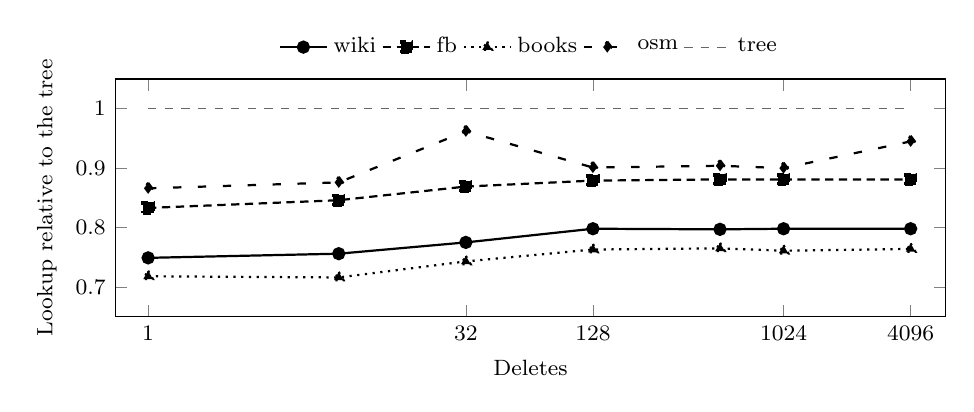
\begin{tikzpicture}
\begin{axis}[
    width=\columnwidth,
    height=4.6cm,
    xmode=log,
    log basis x={2},
    xmin=0.7, xmax=6000,
    ymin=0.65, ymax=1.05,
    xtick={1,32,128,1024,4096},
    xticklabels={1,32,128,1024,$4096$},
    ytick={0.7,0.8,0.9,1.0},
    xlabel={Deletes},
    ylabel={Lookup relative to the tree},
    legend style={at={(0.5,1.05)}, anchor=south, legend columns=5, font=\footnotesize, draw=none, inner sep=1.5pt, cells={anchor=west}},
    tick label style={font=\footnotesize},
    label style={font=\footnotesize},
]
\addplot[black, mark=*, thick] coordinates {(1,0.749) (8,0.756) (32,0.775) (128,0.798) (512,0.797) (1024,0.798) (4096,0.798)};
\addplot[black, mark=square*, densely dashed, thick] coordinates {(1,0.833) (8,0.846) (32,0.869) (128,0.879) (512,0.881) (1024,0.881) (4096,0.881)};
\addplot[black, mark=triangle*, dotted, thick] coordinates {(1,0.718) (8,0.716) (32,0.743) (128,0.763) (512,0.765) (1024,0.761) (4096,0.764)};
\addplot[black, mark=diamond*, loosely dashed, thick] coordinates {(1,0.866) (8,0.876) (32,0.962) (128,0.901) (512,0.904) (1024,0.900) (4096,0.945)};
\addplot[black!60, dashed, line legend] coordinates {(1,1) (4096,1)};
\legend{wiki, fb, books, osm, tree}
\end{axis}
\end{tikzpicture}
\caption{Point lookup after deletes, divided by the history-independent tree in the same run, with the boundary list capped at 32.
A value under 1 is faster than the tree.
The cap is reached at 32 deletes.
Wiki, fb, and books stay near that value through 4{,}096 deletes.
Osm moves from 0.96 at 32 deletes to 0.90 at 128 and 0.95 at 4{,}096.}
\label{fig:slide}
\end{figure}

\subsection{A B+ tree and mixed updates}

Table~\ref{tab:dist} times one uniform delete on a fresh copy, without the run slide.
The rows in Table~\ref{tab:base} are in place on one index.
The B+ tree holds 256 keys in a leaf and has height 4 after the bulk load.
A delete unlinks an empty leaf and leaves the model unbuilt, so the tree is not history independent, and it was not scanned for a retained key.
One million lookups missed nothing.
The median delete is about a microsecond, and the slowest of 512 is 4.9\,$\mu$s on wiki and under 2\,$\mu$s on the other three files.
Lookup on this tree is 760--959\,ns, slower than this index on a fresh arena.

The hashed rank sample draws a rank with exponent $1/(1-0.99)$ and then hashes that rank, which removes the skew, and keeps 512 distinct keys.
It is not a locality workload.
The range sample deletes 512 consecutive keys at the middle of the file.
Both include the slide, with a limit of 32.
The range median on osm is 39.7\,ms, in the slow cluster of Table~\ref{tab:dist}.
The mixed sequence is 20{,}000 single-threaded operations on a fresh index: 16{,}019 lookups, 2{,}017 deletes, and 1{,}964 inserts of keys that were not in the file.
No lookup missed.
An insert that does not fit in its piece shifts the following keys, at most $2^{23}$ of them, into a spare of 4{,}096 keys placed every $2^{23}$ live keys.
That placement is 95 holes on osm.
The boundary list then ended at 32, 32, 54, and 125, so on osm 30 entries sit outside those holes.
The slide does not close a planted spare, and those holes are what the mix lookup searches.
Lookup in that mix was 849\,ns, 1{,}280\,ns, 1{,}066\,ns, and 2{,}141\,ns.
When a spare is used up, a later spare inside the same window is used.
If none remains, the arena is copied with the holes restored, and the piece is copied to the tail only if that copy still cannot open a slot.
The model at the end of this mix matched a fresh build on all four files.

\begin{table}[t]
\caption{B+ tree and in-place deletes on the SOSD files.
B+ lookup is the mean of one million probes.
B+ delete is the median of 512 uniform erases.
Hashed and range are medians of 512 in-place deletes of this index, with the run slide.
Mix is the mean of the deletes and the inserts in a 20{,}000-operation sequence.}
\label{tab:base}
\centering
\footnotesize
\begin{tabular}{@{}lrrrrr@{}}
\toprule
File & B+ ns & B+ $\mu$s & Hashed & Range & Mix del\,/\,ins \\
\midrule
wiki  & 760 & 0.89 & 1.16\,ms & 0.46\,ms & 1.28\,/\,0.22\,ms \\
fb    & 834 & 0.96 & 3.43\,ms & 4.29\,ms & 4.52\,/\,1.96\,ms \\
books & 829 & 0.96 & 2.89\,ms & 1.64\,ms & 3.14\,/\,1.06\,ms \\
osm   & 959 & 1.17 & 12.8\,ms & 39.7\,ms & 26.0\,/\,35.4\,ms \\
\bottomrule
\end{tabular}
\end{table}

\subsection{Limits of the measurement}

There is no WAL, buffer pool, or latch protocol. A log line that names the deleted key would put the key back into durable storage.
Anchor pieces have no density thresholds, so a gap between anchors is still moved linearly.
The exhaustive rank audit missed none of the 1{,}290{,}437{,}010 keys of the fresh arena, and after one middle-key delete it missed none of the 1{,}290{,}437{,}006 survivors.
After 1{,}024 uniform deletes it missed none of 90{,}435{,}987, 199{,}998{,}976, 199{,}998{,}975, and 799{,}998{,}976 survivors.
The timed million-probe check after 1{,}024 deletes is a separate latency measurement.
The 512-delete distribution includes the boundary-list rebuild and leaves out the run slide of Section~\ref{sec:compact}.
The cross-compiler check is the one-input caveat in the design section.
The GCC fuzzer includes the signed shift and the run slide.
ALEX payload retention and ALEX lookup were both measured on the full SOSD files.
LIPP was not given a delete in order to be attacked, lookup timing as a co-tenant side channel was not measured, and the two-snapshot result is recorded and left open.

\section{Discussion}

\subsection{Rebuilding on a timer}

The design that erases the key while keeping the stock index is to replace the index from a fresh build.
A deterministic build is a function of the current keys, so replacing the live model with a fresh static PGM of the packed keys meets the byte condition for that checkpoint.
The question is what a reader of the live model sees before that replacement.
Waiting for the next checkpoint leaves the deleted key in the published model until the rebuild is installed.
On the host in Section~\ref{sec:eval} that rebuild takes 2.30\,s, 7.58\,s, 6.14\,s, and 28.9\,s for wiki, fb, books, and osm.
Dividing those separate builds by the slowest delete in Table~\ref{tab:dist} gives $813\times$, $125\times$, $325\times$, and $156\times$.
Dividing them by the mean delete without the slide, one rebuild costs about as much as 3{,}433 wiki deletes, 3{,}445 fb deletes, 4{,}177 books deletes, and 3{,}798 osm deletes.
A purge larger than that is less work as one rebuild.
The 32-delete batch does not reach that count: on osm it is 25.7\,ms a delete in that earlier binary, and 32 of them are still far under the 28.9\,s rebuild.
A rebuild on every delete makes the wait those full fits, and it reads every surviving key to do it.
Dynamic PGM avoids the wait by inserting a tombstone, and the tombstone is the key.
Delete latency for that call, and for ALEX erase, was not measured: both calls retain the key, so their time is not a time for the byte condition.
The splice publishes the model of the survivors at the end of the call.
The bytes that change stop at the next old start, and the time does not: the call is tens of microseconds on the 200{,}000-key pilot and milliseconds on the full files.
Table~\ref{tab:dist} is the packed-start binary on a copy finished before the clock, with the vacated tail cleared.
A 32-draw on that binary timed the leaf-vector rewrite at 31\,$\mu$s, 536\,$\mu$s, 176\,$\mu$s, and 0.08\,$\mu$s, on 2, 1, 1, and 0 of 32 deletes, while the upper clock was 0.28\,ms, 2.83\,ms, 1.10\,ms, and 4.31\,ms.
In the 32-draw sweep of Table~\ref{tab:modtime}, at $M=0$ the piece move is 24.2\,ms, 53.6\,ms, 54.6\,ms, and 215\,ms of the 24.8\,ms, 56.0\,ms, 55.3\,ms, and 217\,ms means.
At $M=4096$ that move is 2.3\,$\mu$s, 3.2\,$\mu$s, 3.8\,$\mu$s, and 3.8\,$\mu$s, the local fit is 0.27\,ms, 0.16\,ms, 0.18\,ms, and 0.16\,ms, and the rest of the clock is 0.36\,ms, 2.89\,ms, 1.29\,ms, and 5.18\,ms.
The listed parts of one delete do not sum to a mean, because a delete that keeps every leaf start key skips the upper splice entirely.

\begin{table}[t]
\caption{Mean delete time over 32 uniform draws at each anchor modulus.
The copy finishes before the clock, on the shared host of Section~\ref{sec:eval}.
Table~\ref{tab:dist} is the separate 512-draw distribution at $M=4096$.}
\label{tab:modtime}
\centering
\footnotesize
\begin{tabular}{@{}lrrrr@{}}
\toprule
File & $M=0$ & $1024$ & $4096$ & $16384$ \\
\midrule
wiki  & 24.8\,ms & 0.98\,ms & 0.63\,ms & 0.48\,ms \\
fb    & 56.0\,ms & 5.62\,ms & 3.05\,ms & 2.64\,ms \\
books & 55.3\,ms & 3.98\,ms & 1.47\,ms & 0.84\,ms \\
osm   & 217\,ms & 15.1\,ms & 5.34\,ms & 2.40\,ms \\
\bottomrule
\end{tabular}
\end{table}

A million in-place deletes, uniform among the keys still present and with the slide, are Table~\ref{tab:million}.
The counts of 3{,}433, 3{,}445, 4{,}177, and 3{,}798 above leave the slide out.
All four runs cleared the vacated tail, matched a fresh build, and missed no lookup.
Scans of 89{,}437{,}011, 199{,}000{,}000, 198{,}999{,}999, and 799{,}000{,}000 survivors missed none.

\begin{table}[t]
\caption{One million in-place deletes with the slide, uniform among keys still present, on the packed-start binary with the vacated tail cleared.
Lookup is one million probes after the run.
Audit is a scan of every survivor.
The boundary list is the length at the end of the run.
Dividing the static PGM builds of 2.30\,s, 7.58\,s, 6.14\,s, and 28.9\,s by these means gives about 518, 695, 590, and 612.}
\label{tab:million}
\centering
\scriptsize
\begin{tabular}{@{}lrrrr@{}}
\toprule
File & Mean & Tails & Boundaries & Lookup \\
\midrule
wiki  & 4.44\,ms & 264 & 479 & 511\,ns \\
fb    & 10.9\,ms & 242 & 496 & 756\,ns \\
books & 10.4\,ms & 246 & 414 & 625\,ns \\
osm   & 47.2\,ms & 249 & 532 & 918\,ns \\
\bottomrule
\end{tabular}
\end{table}

\section{Conclusion}

Shipped dynamic PGM and ALEX still store a deleted key in the structure erase returns, on generators and on the full SOSD files.
A relative-count splice can make the serialized model match a rebuild before the next packed-key static-PGM checkpoint, and on these files that call finishes sooner than a separate static PGM build.
Two snapshots still name the deleted key for every exact structure we tried.

\bibliographystyle{IEEEtran}
\bibliography{refs}

\section*{Acknowledgment of AI-Generated Content}
An AI coding assistant (Cursor, Grok 4.7) drafted C++ sources, measurement drivers, TikZ figures, tables, and the prose of this manuscript, including the abstract and every numbered section.
The author selected the claims, ran the measurements, edited the text, and is responsible for the content.
PGM-index and ALEX are the public sources of those projects.
The source that produces the tables is the public artifact at https://github.com/koderAP/shi-pla-icde2027.

\end{document}
